\chapter{Theory}
In long and fairly complex reports and articles, especially theoretical and experimental reports where the purpose of the document is to apply, verify, or illustrate one or more theories, include a separate section presenting relevant theoretical formulae and the techniques by which any experimental results are predicted. When introducing equations, be sure to define all symbols used in them.


\section{WPT Architecture}
  Figure {block_diagram} [book] presents the schematic diagram of a general WPT system. The operating principle can be classified into \textit{maximum power transfer} and \textit{maximum power efficiency transfer} [A Critical]. This article is based on the efficiency criterion to reach a compromise between the harvested power and the physical limitation. As suggested in [book], the overall power transmit efficiency $e$ can be decomposed as

\begin{equation}\label{eqn:power_utilization_efficiency}
  e = \frac{{{P_{{\text{dc}},{\text{ST}}}}}}{{P_{{\text{dc}}}^t}} = \underbrace {\frac{{P_{{\text{rf}}}^t}}{{P_{{\text{dc}}}^t}}}_{{e_1}} \cdot \underbrace {\frac{{P_{{\text{rf}}}^r}}{{P_{{\text{rf}}}^t}}}_{{e_2}} \cdot \underbrace {\frac{{P_{{\text{dc}}}^r}}{{P_{{\text{rf}}}^r}}}_{{e_3}} \cdot \underbrace {\frac{{{P_{{\text{dc}},{\text{ST}}}}}}{{P_{{\text{dc}}}^r}}}_{{e_4}}
\end{equation}

where the power transmitter determines the DC-to-RF efficiency ${e_1}$, the channel influences the RF-to-RF efficiency ${e_2}$, the rectenna decides the RF-to-DC efficiency ${e_3}$, and the power management unit (PMU) deals with the DC-to-DC efficiency ${e_4}$. Most existing solutions assume no dependency in between and focus on maximizing each term individually [see ref] then concatenate them together. Specifically, ${e_1}$ ${e_3}$ and ${e_4}$ are often neglected in waveform design and resource allocation. Interestingly, it has been proved by [Communications and][Waveform design][Practical nonlinear] that these efficiencies are coupled with each other, and the problem requires a joint optimization. Indeed, the RF-to-DC efficiency ${e_3}$ is observed to be a nonlinear function of the rectifier input power ${P_{{\text{rf}}}^r}$ [Towards the][Maximum achievable][Power-optimized], which also depends on signal waveform [Optimum waveform][Boosting the]. This article employs a tractable nonlinear harvester model proposed in [Waveform design] that was proved beneficial to the harvested current. 
  
\section{Rectenna Behavior}
  A rectenna receives electromagnetic power with antenna and convert it to electric power with rectifier. Diverse configurations are available for energy harvesting, such as \textit{Schottky} \cite{Akkermans2005, Boaventura2013}, \textit{CMOS} \cite{Stoopman2014, Valenta2014}, \textit{series} \cite{Georgiadis2011, Collado2013}, \textit{shunt} \cite{McSpadden1998, Guo2012}. Interestingly, those models are not equally suitable for the same input power, and maximizing the rectenna efficiency ${e_3}$ requires a proper selection according to the power range. As reported in \cite{Valenta2014, Costanzo2016}, low barrier Schottky diodes are commonly used for input power between \SI{1}{\uW} and \SI{1}{\mW}. Specifically, single diode is preferred for low power below \SI{500}{\uW} and multiple diodes are typically applied for input power above \SI{500}{\uW} \cite{Clerckx2019}. Hybrid designs as \cite{Sun2013} may be employed to maintain a high efficiency for large power range.

Besides the rectenna model, the shape of the received signal also influences the RF-to-DC efficiency ${e_3}$. It was first demonstrated in \cite{Trotter2009} that multisine waveform \textit{i.e. Power-Optimized waveform (POW)} outperforms the single tone waveform \textit{i.e. Continuous Wave (CW)} in operation range and power efficiency. The expression of a multisine waveform with $N$ subcarriers writes as a summation of $N$ sine waves:

\begin{equation}\label{eqn:multisine}
  {V_{{\text{multisine}}}}(t) = \sum\limits_{n = 0}^{N - 1} {\frac{1}{{\sqrt N }}} \sin \left( {2\pi \left( {{f_{\text{0}}} + n\Delta f} \right)t} \right)
\end{equation}

where ${{f_{\text{0}}}}$ is the minimum frequency and ${\Delta f}$ is the spacing. Figure \ref{fig:waveform_comparison} \cite{Trotter2009} illustrates the three-subcarrier case for both signals in time and frequency domains. It can be observed that multisine waveform provides a higher PAPR equals to ${\sqrt N }$ and occupies a bandwidth of $(N - 1) \Delta f$ with the same average power as CW, which is equally distributed to its components.

\begin{figure}
  \centering

  \begin{subfigure}{.45\textwidth}
    \centering
      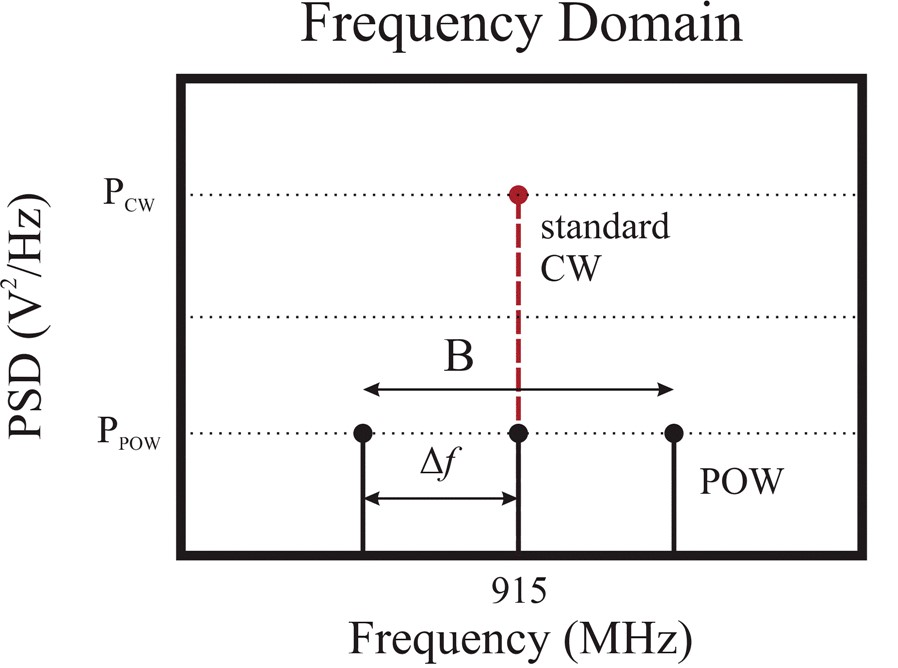
\includegraphics[width=\textwidth]{waveform_frequency_domain}
    \caption{Frequency domain}
    \label{fig:waveform_frequency_domain}
  \end{subfigure}
  \begin{subfigure}{.45\textwidth}
    \centering
      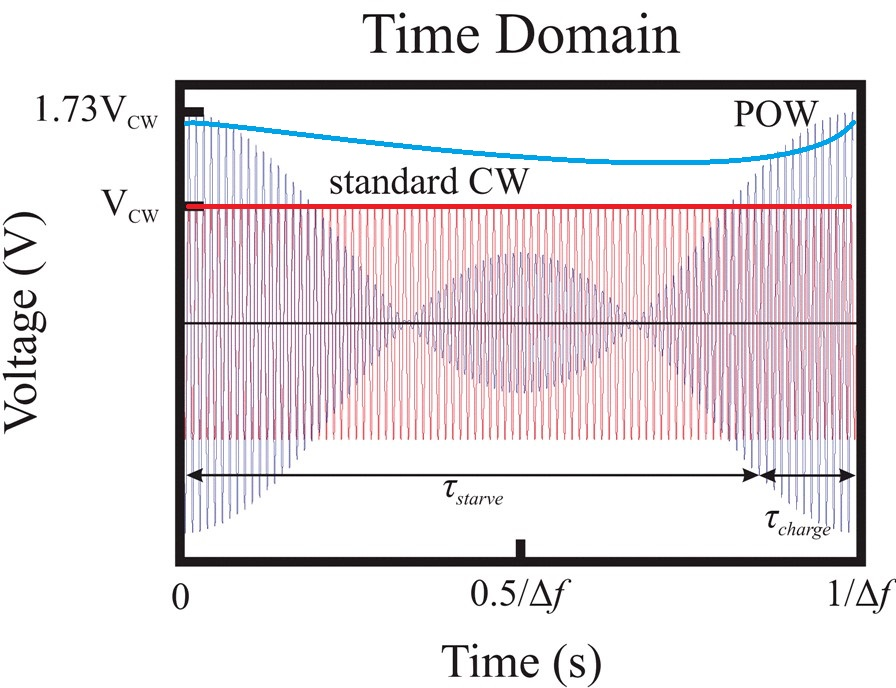
\includegraphics[width=\textwidth]{waveform_time_domain}
    \caption{Time domain}
    \label{fig:waveform_time_domain}
  \end{subfigure}

  \caption{Comparison of a typical 3-subcarrier multisine and CW in time and frequency domains (modified from \cite{Trotter2009}). The thick lines are examples of rectifier output voltage.}
  \label{fig:waveform_comparison}
\end{figure}

The advantage of multisine in WPT is that the high PAPR increases the peak rectifier output voltage. With a proper signal and circuit design, high voltage may be preserved during the cycle if discharging is slow enough, as indicated by the thick blue line in Figure \ref{fig:waveform_time_domain}. To enhance the harvested power, a large number of tones may be used to increase PAPR, and the multisine signal will appear as pulses with period of $1/\Delta f$. Most of the signal power will be concentrated in those pulses to trigger the diode and charge the capacitor. However, more subbands can lead to smaller frequency gaps and longer charging cycle when the bandwidth is fixed.

It can be hard to derive an accurate expression of the RF-to-DC efficiency ${e_3}$ on the power and shape of the rectifier input signal, as practical energy harvesting circuits consists of various nonlinear components as diodes, capacitors and inductors. It is also sensitive to parasitic sources, impedance matching, and harmonic generation \cite{Strassner2013, Valenta2014}. In this article, we employ the \textit{diode linear model} and \textit{diode nonlinear model} proposed in \cite{Clerckx2016} based on the diode current-voltage (I-V) characteristics to capture the fundamental pattern of rectenna and investigate its impact on resource allocation and system design. A superposed waveform containing modulated information and multisine power components is optimized according to CSI on top of both models.

  
\section{Analytical Rectenna Model}
  As illustrated by Figure \ref{fig:rectenna_circuit}, the rectifier consists of a single diode as the source of nonlinearity and a low-pass filter to store energy.

\begin{figure}
  \centering
    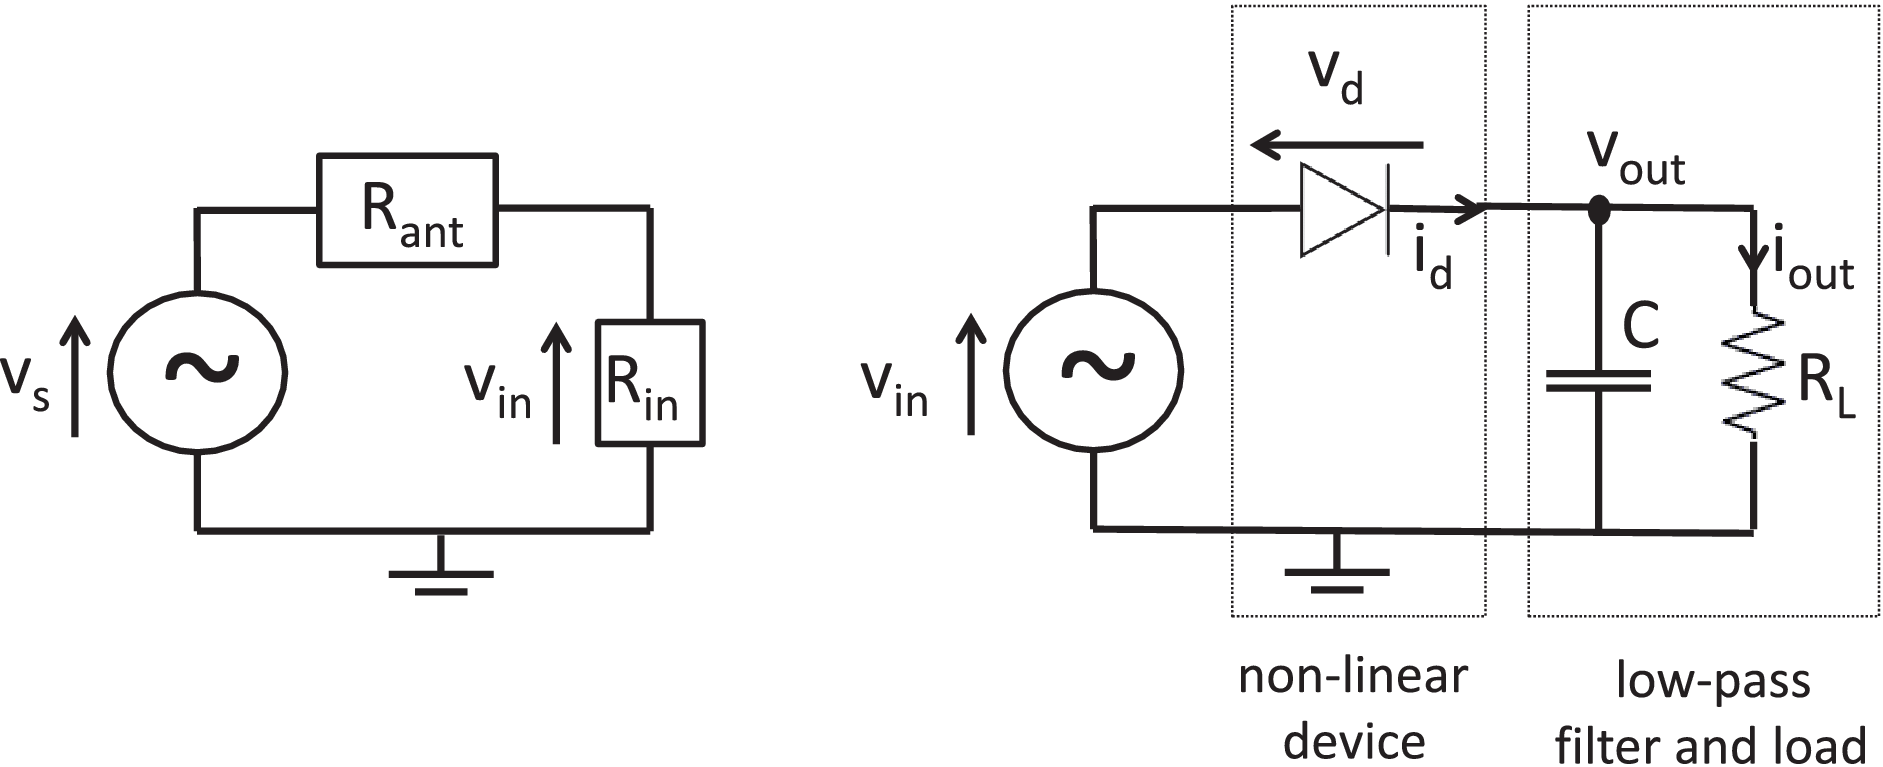
\includegraphics[width=\textwidth]{rectenna_circuit}
  \caption{Rectenna equivalent circuit (left) and a single diode rectifier (right) \cite{Clerckx2018a}}
  \label{fig:rectenna_circuit}
\end{figure} 

Assume lossless, the equivalent circuit includes a voltage source ${v_{\text{s}}}(t)$ connected to a series antenna impedance ${Z_{{\text{ant}}}} = {R_{{\text{ant}}}} + j{X_{{\text{ant}}}}$ followed by a combined impedance of the rectifier and the matching network ${Z_{{\text{in}}}} = {R_{{\text{in}}}} + j{X_{{\text{in}}}}$. The perfect matching condition is

\begin{equation}\label{eqn:perfect_match}
  {R_{{\text{in}}}} = {R_{{\text{ant}}}},{X_{{\text{in}}}} =  - {X_{{\text{ant}}}}
\end{equation}

When equation \ref{eqn:perfect_match} is satisfied, the rectifier input voltage equals 

\begin{equation}\label{eqn:rectifier_input_voltage}
  {v_{{\text{in}}}}(t) = {v_{\text{s}}}(t)/2 = y(t)\sqrt {{R_{{\text{in}}}}} 
\end{equation}

and the input power to the rectifier writes 

\begin{equation}\label{eqn:rectifier_input_power}
  P_{{\text{rf}}}^r = \mathbb{E}\left[ {y{{(t)}^2}} \right] = \mathbb{E}\left[ {{v_{{\text{in}}}}{{(t)}^2}} \right]/{R_{{\text{in}}}}
\end{equation}

It is also assumed that the noise is too small to be harvested.
